\documentclass[10pt,a4paper]{article}
\usepackage[utf8]{inputenc}
\usepackage{amsmath}
\usepackage{amsfonts}
\usepackage{amssymb}
\usepackage{graphicx}
\usepackage{url}

\title{Recognition of text in images \\ Project proposal}
\author{Johnny CHEN, Haotian CHU, Marouen CHAFROUDA}
\date{\today}

\begin{document}
\maketitle

\section{Problem definition and motivation}
The problem is the following: Having as input an image with some text, we want to be able to extract the words written on it, not just detecting the bounding box of the word, but what letters, what words compose the text.

Our first thoughts about the context:
\begin{itemize}
	\item We could first restrict the language of the text to english, and see later if the language 			affects the result.
	\item Different kind of images could be used: wild ones or more structured ones:
		\begin{center}
			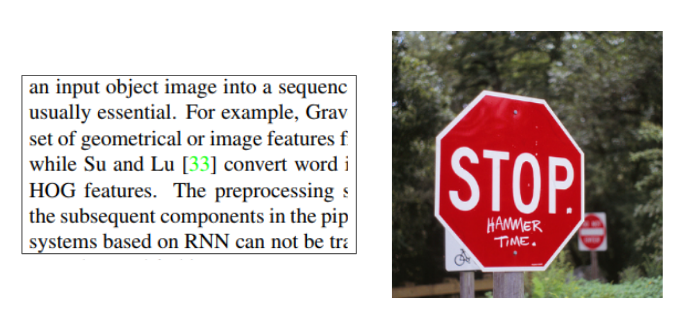
\includegraphics[scale=0.5]{wild_image_ex.png}
		\end{center}
	\item start with simple images: just one word per image first.
\end{itemize}

Text recognition, or rather OCR for Optical Character Recognition, has been studied from a very long time ago, ever since the 20th century. It has both computer vision focused solutions and deep learning focused solutions. 

Text recognition has great use in travelers' everyday lives. For exemple, at the restaurant faced with a lot of unknown foreign words, instead of trying to translate every word, you could just image it and extract all the words, then combine it with Natural language processing such as translation to have a rapid translation. It is even more useful if you are not used to writing foreign words.

There are already mobiles apps developped for that, though most of them have to focus on one word at a time.


We think this could be a good project in order to put into practice our computer vision knowledge learned in class. The idea is not to have an application which has high performance, but rather to understand the concepts of computer vision behind, try to implement those concepts, and see their influence.


\section{Methodology}
Our principal focus will be to understand the theory behind first, and then try to implement each part of the theory with Python. As there is no available code, we will have to implement everything from scratch.

The papers proposes classical steps in computer vision:
\begin{itemize}
\item pre-processing such as de-noising
\item edge detection using for exemple sobel operator
\item Selective local thresholding 
\item Text area enhancement 
\item Coarse-to-fine detection 
\end{itemize}
\section{Dataset}
For now, we don't have specific datasets, but we could look into datasets such as:
SVHN, license plates, MNIST

\section{Evaluation}
For now, we don't have any metrics besides visualisation.

\section{Reference}
\begin{itemize}
\item "A NEW APPROACH FOR VIDEO TEXT DETECTION" \\
\url{https://ieeexplore.ieee.org/stamp/stamp.jsp?tp=&arnumber=1037973&tag=1}

\item "A Technical Review on Text Recognition from Images" \\
\url{\https://www.researchgate.net/publication/274838198_A_Technical_Review_on_Text_Recognition_from_Images}
\end{itemize}

\end{document}
